\providecommand{\main}{..}
\documentclass[\main/master.tex]{subfiles}
\begin{document}
\chapter{introduction}\label{chp:example-1}
\section{garvity measurement problem}

Gravitational field has a very unique nature compare to other fields. Gravitational field could not be shielded and the force could not be compensated. The Gravitational force is inverse to the square of the distance between the masses, causing a very weak force.Those properties makes it a dominating force in nature but very hard to measure at experiments.
\par
The first modern gravimeter was invented in 1936.Precision gravimetry could defined as obtaining repeatability the strength of a gravitational field at high precision. Gravimetry is used to exam the matter properties or the gravitational field.
\par 
Most measuring methods, rely on the Cavendish experiment, first performed in the 17th century. The measuring methods use a torsional pendulum and measure the spectral density of the gravitational field. These methods have precision and accuracy limitations especialy at low frequencies.
\par
Precision gravimetry extensively used at oil and gas exploration \cite{Bell98}, mining \cite{Leeuwen00}, mapping earth’s local gravity and temporal geological shifts. Determining Newton’s  gravitational constant and gravitational imaging systems.  


is used extensively in mapping the earth's local gravity \cite{Wahr04,Bingham10}, oil and gas exploration \cite{Bell98}, mining \cite{Leeuwen00}, mapping temporal geological shifts, the determination of Newton's gravitational constant \cite{Luther82, Kuroda95, Karagioz96, Bagley97, Gundlach00, Quinn01, Armstrong03, Kleinevoss99, Parks10, Peters99, Mcguirk02, Dimopoulos07, Lamporesi08, Sorrentino10, Rosi14} and gravitationally imaging opaque systems.


%\par
%Precision of the order of 1μg (1 g = 9.8 m s−2to 1nano-g) are often used for mapping geological variations. Both relative and absolute measurements are employed


\doublespacing
\hspace{5 mm} This is a \LaTeX template for preparing a dissertation according to the University of Rochester guidelines \cite{uofr_guidelines} as of July 2020. It also includes some useful \LaTeX formatting including a working example of a bibliography. You will need a working TeX distribution such as MikTeX \cite{miktex_home} or TeXLive \cite{texlive_nodate} to compile this document.  \par
Here is an example equation (from \cite{einstein1905tragheit} \cite{jordan2015heisenberg} ) that has it's own label we will reference in Chapter~\ref{chp:example-2}:
\begin{equation}
E=mc^{2}.\label{eqn:energy-mass-equivalence-relation}
\end{equation}
Here is an example image:
\begin{figure}[htbp]
	\centering
	\fbox{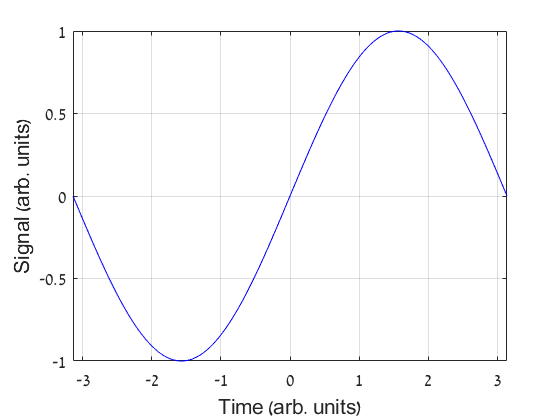
\includegraphics[scale=0.5]{\main/images/chapter_1_example/img_example.png}}
	\caption[Example Image]{Example Image. This image is also labeled internally so we can reference it throughout the text.}
	\label{fig:sine-wave}
\end{figure}
If you want to reference the example figure (Fig.~\ref{fig:sine-wave}), you can. See also Fig.~\ref{fig:cosine-wave}.


\end{document}